\documentclass{article}

\usepackage{graphicx}
\usepackage{booktabs}
\usepackage{longtable}
\usepackage{tabu}
\usepackage{listings}
\usepackage{hyperref}
\usepackage{tcolorbox}
\usepackage{neurips_2019}
\usepackage[utf8]{inputenc}
\usepackage[T1]{fontenc}
\usepackage{url}
\usepackage{amsfonts}
\usepackage{nicefrac}
\usepackage{microtype}

\setlength\parindent{0pt}

\title{DQN-DDQN agent performance}

\author{%
anjanav24
}

\begin{document}

\maketitle

\section{Section 1}

\begin{figure}[!htb]
\minipage{0.49\textwidth}
\includegraphics[width=\linewidth]{charts/Section-2-Panel-0-zc608kppa}
\caption{}
\endminipage\hfill
\minipage{0.49\textwidth}
\includegraphics[width=\linewidth]{charts/Section-2-Panel-1-fbmu1nz2p}
\caption{}
\endminipage
\end{figure}

\begin{figure}[!htb]
\minipage{0.49\textwidth}
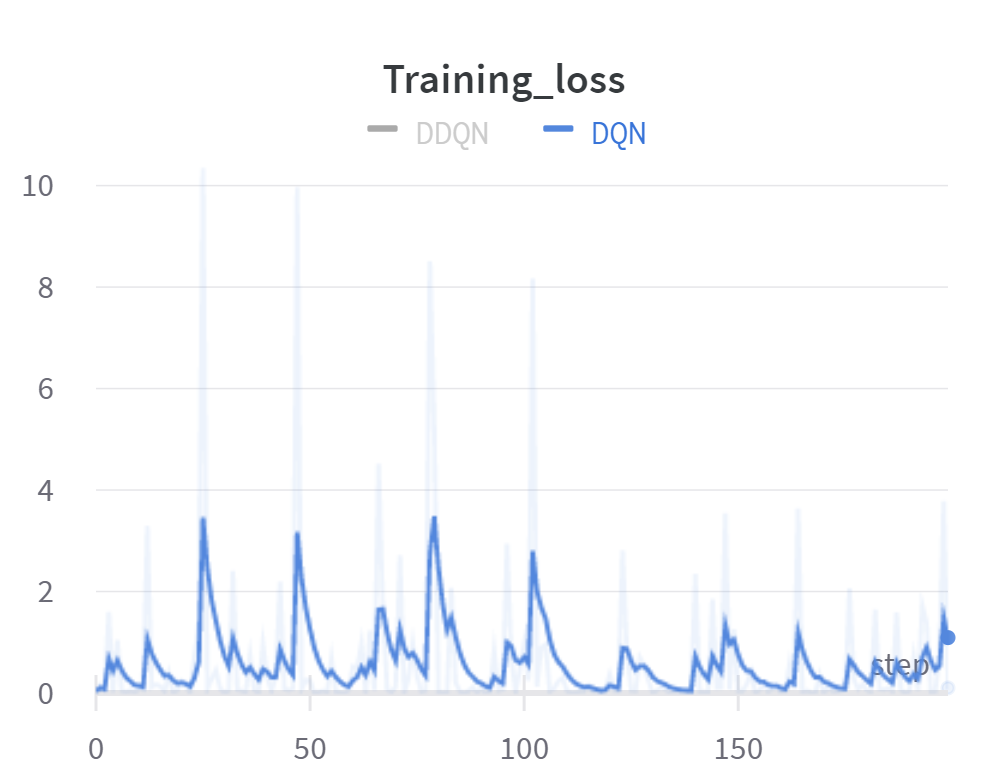
\includegraphics[width=\linewidth]{charts/Section-2-Panel-2-77zytmx3y}
\caption{}
\endminipage\hfill
\minipage{0.49\textwidth}
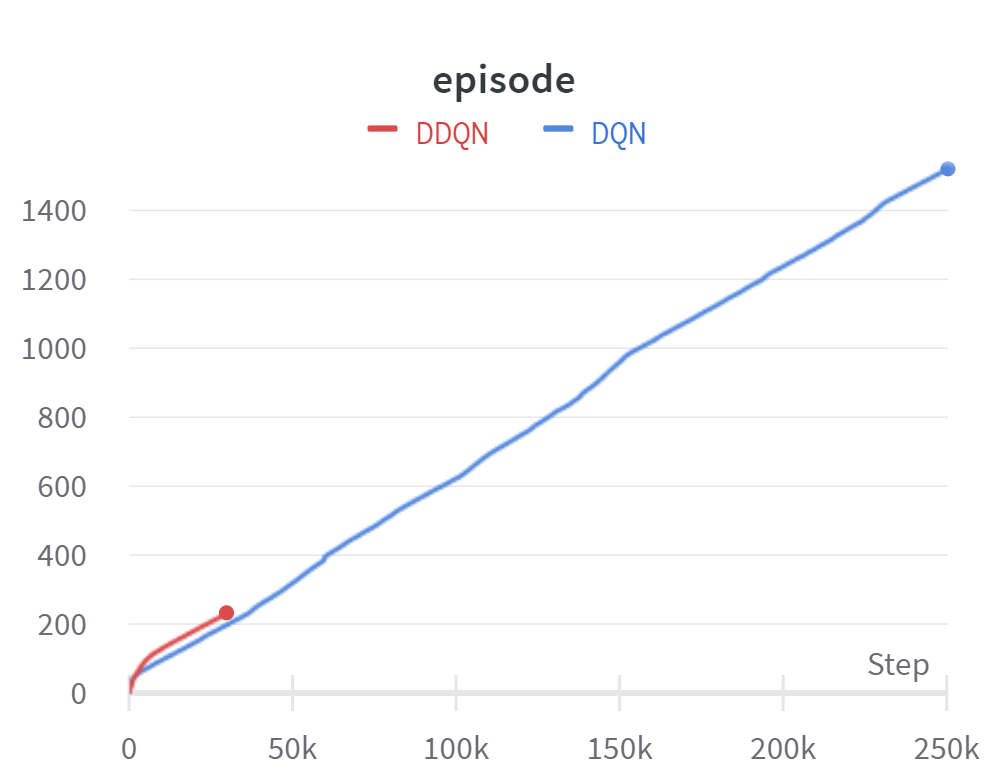
\includegraphics[width=\linewidth]{charts/Section-2-Panel-3-tdwehebrh}
\caption{}
\endminipage
\end{figure}

\begin{figure}[!htb]
\minipage{0.49\textwidth}
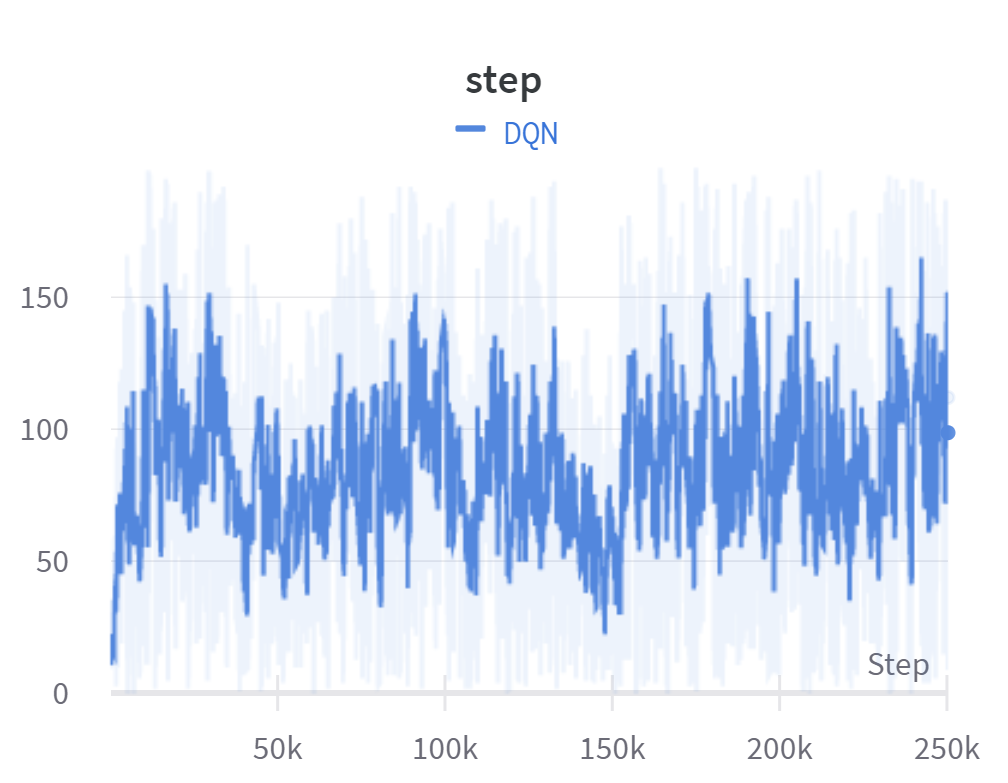
\includegraphics[width=\linewidth]{charts/Section-2-Panel-4-nz8ry0kxx}
\caption{}
\endminipage
\end{figure}

\nocite{*}
\bibliographystyle{unsrt}
\bibliography{bibliography}
\end{document}